\section{Características del Robot} \label{sec:caracteristicas_del_robot}

Antes de desarrollar la tabla de información principal del robot, se hizo el diagrama de Denavit Hartenberg como guía visual. En este se colocan los ejes Z y X de rotación, así como las distancias de cada eslabón y los tipos de articulación. 

\begin{figure}[H]
    \centering
    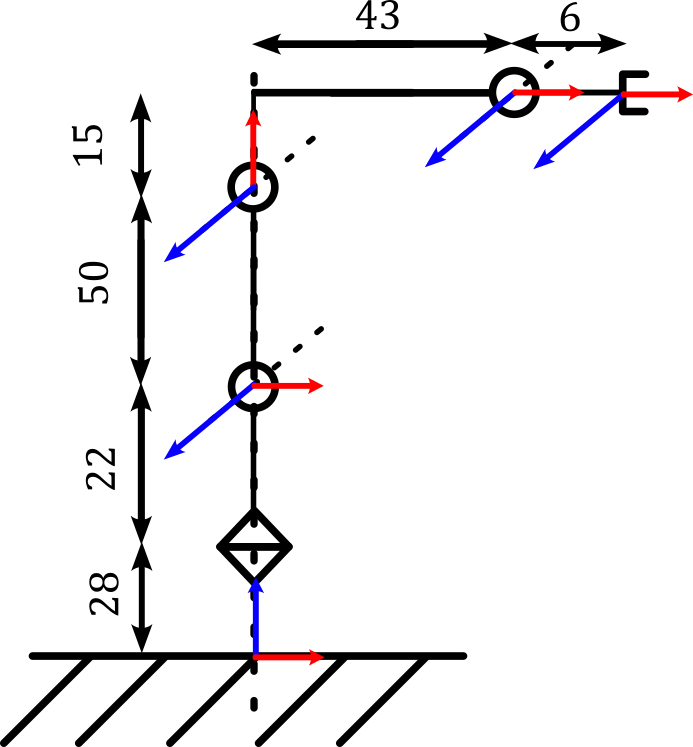
\includegraphics[width=0.3\textwidth]{img/robotFinal.png}
    \caption{Diagrama DH Robot}
    \label{fig:robotDH}
\end{figure}

La tabla de información principal se completa utilizando la regla de la mano derecha para conocer el sentido de cada rotación. Además, se colocan las restricciones para cada articulación, considerando si son rotacionales o prismaticas. 
\pagebreak

\begin{table}[H]
    \centering
    \begin{tabular}{|c|c|c|c|c|c|c|c|c|c|c|c|c|}
    \hline
    \textbf{N} & \textbf{$\theta$} & \textbf{d} & \textbf{a} & \textbf{$\alpha$} & \textbf{tipo} & \textbf{$q_{min}$} & \textbf{$q_{max}$} & \textbf{$\dot{q}_{max}$} & \textbf{$\ddot{q}_{max}$} & \textbf{$\tau$} & \textbf{$\mu_s$} & \textbf{$\mu_k$} \\
    \hline
    1 & 0   & 50 & 0  & -90 & r & -180 & 180 & 180 & 360 & 134 & 0.1 & 0.2 \\
    2 & 90  & 0  & 50 & 0   & r & -90  & 90  & 180 & 360 & 110 & 0.1 & 0.2 \\
    3 & -90 & 0  & 43 & 0   & r & -90  & 90  & 180 & 360 & 50  & 0.1 & 0.2 \\
    4 & 0   & 0  & 6  & 0   & r & -90  & 90  & 180 & 360 & 19  & 0.1 & 0.2 \\
    \hline
\end{tabular}
\caption{Parámetros DH del robot junto con límites articulares y características dinámicas}
\label{tab:tabla_dh_completa}
\end{table}

\bigskip
\noindent
\textbf{Donde (cambien las unidades):}
\begin{description}
	\item[N] Número de la articulación.
	\item[\(\theta\)] Ángulo articular (grados).
	\item[\(d\)] Desplazamiento articular (centímetros).
	\item[\(a\)] Longitud del eslabón (centímetros).
	\item[\(\alpha\)] Ángulo de torsión DH (grados).
	\item[tipo] ‘r’ para articulación rotacional, ‘p’ para prismática.
	\item[\(q_{\min}\), \(q_{\max}\)] Límites de posición (grados o unidades de desplazamiento).
	\item[\(\dot q_{\max}\)] Límite de velocidad (grados/s).
	\item[\(\ddot q_{\max}\)] Límite de aceleración (grados/s²).
	\item[\(\tau\)] Torque o fuerza máxima permitido (\(N \cdot m\) o \(N\)).
	\item[\(\mu_s\)] Fricción estática (\(N\) o \(N \cdot m\)).
	\item[\(\mu_k\)] Fricción cinética (\(N \cdot m \cdot s\) o \(\frac{N \cdot m \cdot s}{rad}\)).
\end{description}

